\documentclass[IJ]{cesj}
\usepackage{graphicx}
\usepackage{listings}

\author{Ga\"etan Lehmann}
\institute{Biologie du d\'eveloppement et de la reproduction, INRA de Jouy-en-Josas}

\title{MinimaImpositionImageFilter}
\abstract{A filter to impose to the input image the minima defined in the marker image}
\keyword{minima imposition, mathematical morphology}
\year{2005}

\leftmark{Ga\"etan Lehmann}
\rightmark{Ga\"etan Lehmann}

\begin{document}
\lstset{language=c++}
\maketitle
% \tableofcontents

\section{Description}
MinimaImpositionImageFilter is a filter to impose a set of minima defined in the marker image to the input image. It may be used with the watershed filter to perform a marker-controlled segmentation.

\section{Implementation}
MinimaImpositionImageFilter is implemented as a sequence of filters.

\section{Usage}
Import the header
\begin{lstlisting}
#include "itkMinimaImpositionImageFilter.h"
\end{lstlisting}
Create the filter
\begin{lstlisting}
typedef itk::MinimaImpositionImageFilter< IType, IType > FilterType;
FilterType::Pointer filter = FilterType::New();
\end{lstlisting}
MinimaImpositionImageFilter requires an input image, and a marker image which defines the minima to impose. All non zero pixels in the marker image are minima to impose.
\begin{lstlisting}
filter->SetInput( reader->GetOutput() );
filter->SetMarkerImage( reader2->GetOutput() );
\end{lstlisting}
During the minima imposition, the image is shifted by 1 by default to avoid having to markers in the same minima. However, the default value may not be relevant in some cases and can thus be modified with the SetShift() method.
\begin{lstlisting}
filter->SetShift( 1 );
\end{lstlisting}
MinimaImpositionImageFilter is a connected component filter. Whith the SetFullyConnected() method, the user can define whether the connected components are defined strictly by face connectivity or by face+edge+vertex connectivity.
\begin{lstlisting}
filter->SetFullyConnected( true );
\end{lstlisting}

\section{Example}
The Figure~\ref{input} show the input image in gray, and a single user defined marker in red. The Figure~\ref{output} is the output of the filter.

\begin{figure}[hb]
\centering
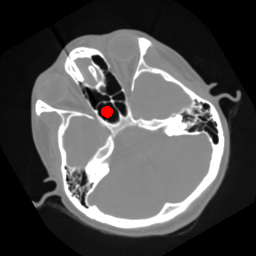
\includegraphics[width=0.5\textwidth]{cthead1}
\caption{The input image together with the marker (in red).\label{input}}
\end{figure}

\begin{figure}[hb]
\centering
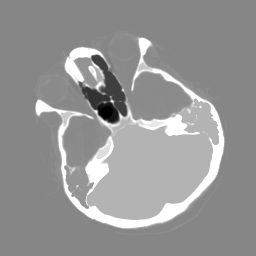
\includegraphics[width=0.5\textwidth]{test}
\caption{The output image.\label{output}}
\end{figure}

\end{document}
